% Joshua Reed
% Fall, 2017
% 
% hw1.tex
% 
% Homework for random processes.

% chktex-file 1 chktex-file 13 chktex-file 25 chktex-file 3 chktex-file 36

\documentclass[12pt]{article}
\usepackage[margin=1in]{geometry} 
\usepackage{amsmath,amsthm,amssymb}
\usepackage{pgfplots}
\usepackage{listings}
\usepackage[compact]{titlesec}
\usepackage{graphicx}
\graphicspath{{img/}}

\setlength\parindent{0pt}
\setlength{\parskip}{\baselineskip}
\titlespacing{\section}{0pt}{5pt}{-\parskip}
\titlespacing{\subsection}{0pt}{-5pt}{-\parskip}
\titlespacing{\subsubsection}{0pt}{-8pt}{-\parskip}


\makeatletter
\renewcommand{\@seccntformat}[1]{}
\makeatother

% For Align:
%'*' tells LaTeX not to number lines.
%Align is a math environment. Thus \text{} is used for text contained within.
%'&' indicates a seperation between columns.

\begin{document}

{%Header section
  \large \bfseries 
  Joshua Reed \\
  Fall, 2017 \\
  \begin{center}
    {\huge Homework 1}\\
    EE 520 - Random Processes \\% chktex 8 
  \normalsize Problems: 1.1, 1.4, 1.9, 1.27, 1.31, 1.35, 1.49, 1.63, 1.65
  \end{center}}
 
 
\section{1.1} 
\subsection{Exercise}
For `Ralph is probably guilty of theft'' to have meaning in the relative frequency 
approach to probability, what data is needed?

\subsection{Solution}
\subsubsection{Relative Frequency}
Relative Frequency is how often something happens divided by the total number of outcomes.

\subsubsection{What data is needed for the above statement?}
We would need to know something like the number of times Ralph was guilty of theft when accused. 

If Ralph was guilty the last 3 times he was accused, and he's been accused 4 times, then the 
above statemnt would seem reasonable. Ralph has in the past shown himself to be 75\% likely 
to be guiltly of theft when accused.

\section{1.4} 
\subsection{Exercise}
A fair coin is flipped three times. What is the probability of two heads and one tail?

\subsection{Solution}
\subsubsection{Sample Space for One Coin Toss}
$\Omega = \{H, T\}$

\subsubsection{Sample Space for Two Coin Tosses}
$\Omega = \{(H,H), (T,T), (T,H), (H,T)\}$

\subsubsection{Sample Space for Three Coin Tosses}
\begin{align*}
\Omega  = \{ &(H,H,H), (H,H,T), (H,T,H), (H,T,T) \\
&(T,T,T),(T,T,H),(T,H,T),(T,H,H)\} 
\end{align*}


\subsubsection{Sample Space for n Coin Tosses}
Because each coin can either be heads or tails, each coin toss increases the number of possible outcomes by a factor of 2. 

Thus, $|\Omega| = 2^n$.

\subsubsection{Number of Ways to Flip Two Heads and a Tail}
In this case because there is only one tail, this is simply a question of how many places can the tail be placed?

For example the outcome (H,T,H) places the T in the second Trial.

Here there are three places for T to be placed. Thus 3 ways to get exactly one tail. $|E| = 3$.

\subsubsection{Probability of Two Heads and a Tail}
\begin{align*}
P(E) &= \frac{|E|}{|\Omega|}\\
&= \frac{3}{8}
\end{align*}

\section{1.9}
\subsection{Exercise}
Four equally likely outcomes $\zeta_1, \zeta_2, \zeta_3$, and $\zeta_4$, and two 
events $A=\{\zeta_1,\zeta_2\}$ and $B=\{\zeta_2,\zeta_3\}$. Express $AB^c, BA^c, AB$, 
and$ A\cup B$ in terms of their elements (outcomes).

\subsection{Solution}
\subsubsection{$A^c$ and $B^c$}
$A^c =\{\zeta_3, \zeta_4\}\\
B^c = \{\zeta_1, \zeta_2\}$

\subsubsection{$AB^c$}
\begin{align*}
AB^c &= \{\zeta_1, \zeta_2\} \cap \{\zeta_1, \zeta_2\}\\
&= \{\zeta_1, \zeta_2\}
\end{align*}

\subsubsection{$BA^c$}
\begin{align*}
BA^c & = \{\zeta_3, \zeta_4\} \cap \{\zeta_3, \zeta_4\}\\
 &= \{\zeta_3, \zeta_4\}
\end{align*}

\subsubsection{$AB$}
$AB = \emptyset$

\subsubsection{$A \cup B$}
\begin{align*}
AB &= \{\zeta_1, \zeta_2\} \cup \{\zeta_1, \zeta_2\}\\
& = \{\zeta_1, \zeta_2\, \zeta_3, \zeta_4\}
\end{align*}








\section{1.27}
\subsection{Exercise}
From a regular deck, are the events: A: Selecting an ace, and B: selecting a red card independent?

\subsection{Solution}
\subsubsection{Rule for Independent Events}
$P(A \cap B) = P(A)P(B)$

\subsubsection{Probability of Selecting an Ace}
\begin{align*}
P(A) & = \frac{4}{52}\\
& = \frac{1}{13}
\end{align*}

\subsubsection{Probability of Selecting a Red Card}
\begin{align*}
P(A) & = \frac{26}{52}\\
& = \frac{1}{2}
\end{align*}

\subsubsection{Probability of Selecting a Red Ace}
\begin{align*}
P(A) & = \frac{2}{52}\\
& = \frac{1}{26}
\end{align*}

\subsubsection{Check for Indepence}
\begin{align*}
P(A \cap B) & \stackrel{?}{=} P(A)P(B)\\
\frac{1}{26}& \stackrel{?}{=} (\frac{1}{2})(\frac{1}{13})\\
& \stackrel{\checkmark}{=} \frac{1}{26}
\end{align*}

These events are independent.

\section{1.31}
\subsection{Exercise}
Which probability is greater, the probability that she works as an office manager or the probability that she is an office
manager who is active in nature-defense organizations?

\subsection{Solution}
\subsubsection{Hedging Bets}
There are so many variables concernign this situation. 

\subsubsection{Answer}
In this case, being active in nature-defense organizations and being an office
manager is a subset of just being an office mangager. Therefore, the chance that 
she is both is less or equally as likely at most.

\section{1.35}
\subsection{Exercise}
Assume there are 3 machines A, B, and C. Each produces 25, 35, and 40 percent 
of the chips made respectively. Of their 
outputs, 5, 4, and 2 percent of the chips are defective. A chip is 
drawn and found defective. What is the probability that 
this chip was manufactured by machine A, B, and C?

\subsection{Solution}
\subsubsection{Total Number of Defective Chips}
For every hundred chips produced, each machine produces:\\
$A=0.05*25=1.25$,\\ 
$B=0.04*35=1.4$,\\
$C=0.02*40=0.8$.

$Total=0.8+1.25+1.4=3.45$
\subsubsection{Probability Per Machine}
\begin{align*}
A&=\frac{1.25}{3.45}\\ 
&=0.36\\
B&=\frac{1.4}{3.45}\\ 
&=0.41\\
C&=\frac{0.8}{3.45}\\
&=0.23
\end{align*}  

\section{1.49}
\subsection{Exercise}
One diamond per 1000 beads. An inspecter inspects 100 beads, what is the 
probability that the smuggler gets caught?

\subsection{Solution}
\subsubsection{Assumption}
To make the problem easier, I'm going to assume there is 1 diamond for 
every 999 beads. The wording of the problem is a bit ambiguous.

Also, I'm going to treat the problem as though there is an infinite number of 
beads and diamonds. Thus removing one does not affect the probability of 
checking the next bead.

\subsubsection{Binomial Trials}
Let $X$ be the number of successes in $n$ trials.\\
Further, let p be the probability of success.\\
$P(X=k)=\binom{n}{k}p^k(1-p)^{n-k}$ \\
where $\binom{n}{k} = \frac{n!}{k!(n-k)!}$

\subsubsection{Related to this Case}
Here the binomial formula is applied because the probability of the smuggler being caught is the 
probabilty of getting 1 or more successes in 100 trials.

\begin{align*}
P(X\geq1) &=\sum_{k=1}^{100}P(X=k)\\
&=\sum_{k=1}^{100}\binom{100}{k}p^k(1-p)^{100-k}
\end{align*}

According to Wolfram Alpha, this comes to 0.09521.

Another way to compute this would be to find the probability of exactly 0 successes and take the compliment.

\begin{align*}
1-P(X=0) &=1-P(X=0)\\
&=1-\binom{100}{0}p^0(1-p)^{100-0}\\
&=1-(1)(1)(1-\frac{1}{1000})^{100}\\
&=1-(\frac{999}{1000})^{100}\\
&=1-0.9048\\
&=0.09521
\end{align*}




\section{1.63}
\subsection{Exercise}
The average number of cars arriving at a tollbooth is $\lambda$ cars per minute and the probability of cars arriving 
is assumed to follow the Poisson law. Given that five cars arrive in the first two minutes, what is the probabiltiy of 10
cars arriving in the first four minutes?

\subsection{Solution}
\subsubsection{Poisson Law}
X is the number of arrivals in time  t. $\lambda$ is the arrival rate.

$P(X=k) = \frac{(\lambda t)^k}{k!}e^{\lambda t}$

\subsubsection{Related to this Problem}
Currently we have 5 cars in two minutes. $\lambda$ is in cars per minute. It seems that the question is really asking
what is the probability of 5 more cars in the next two minutes.

$P(X=5) = \frac{(2 \lambda)^5}{5!}e^{2 \lambda}$

\subsubsection{Extrapolating}
To find lamda, the average number of cars per minute\ldots
\begin{align*}
\lambda = \frac{5 cars}{2 minutes}
\lambda = \frac{2.5 cars}{1 minutes}
\end{align*}

\begin{align*}
P(X=5) &= \frac{(5)^5}{5!}e^{5}\\
 &= \frac{625}{4}e^{5}\\
\end{align*}

This doesn't seem quite right. I'll ask about this in class.

\section{1.65}
\subsection{Exercise}
Assume that code errors in a computer program occur as follows: A line of code contains errors with probability p=0.001 and
is error free with probability q=0.999. Also errors in different lines occur independently. In a 1000-line program what 
is the approximate probability of finding 2 or more erroneous lines?

\subsection{Solution}
\subsubsection{Binomial Trials}
$P(X=k)=\binom{n}{k}p^k(1-p)^{n-k}$ \\

\subsubsection{Related to this Problem}
This can be computed as the complement of finding 1 or fewer lines of code in error.
\begin{align*}
P(X\geq2)&=1-P(X=0)-P(X=1)\\
&=1-\binom{1000}{0}0.001^0(1-0.001)^{1000-0}-\binom{1000}{1}0.001^1(1-0.001)^{1000-1}\\
&=1-(1)(1)(0.999)^{1000}-(1000)0.001(0.999)^{1000-1}\\
&=1-(0.999)^{1000}-(1000)0.001(0.999)^{999}\\
&=0.264\\
\end{align*}


\section{Python Die Problem}
\subsection{Exercise}
Each player either gets 10 or 15 die. These die have 2 sides with dots and 4 without. 
Plot a distribution $P(s<K)$. 
\subsubsection{Question A}
How many dots would be required such that most $(>50\%)$ players fail to roll that many dots?
\subsubsection{Question B}
What is the minimum number of dots that will be showing for 90\% of rolls? Explain.

\subsection{Solution}
\subsubsection{View of the Problem}
Each die has a chance of success of 1/3. Rolling 10 or 15 of these die would be a binomial distribution.

\subsubsection{Binomial Probability}
The probabilty of X successes in n trials with probability of success p.\\
 b(X,n,p)\\
$P(X=k)=\binom{n}{k}p^k(1-p)^{n-k}$

\subsubsection{As Applied}
\begin{align*}
P(X<k)&=\binom{10}{k}(1/3)^k(1-1/3)^{10-k}\\
&=\binom{10}{k}(1/3)^k(2/3)^{10-k}
\end{align*}

\subsubsection{Python Code and Plot}
\lstset{language=Python}
\lstset{frame=lines}
\lstset{caption={Python Plot Code}}
\lstset{label={lst:code_direct}}
\lstset{basicstyle=\footnotesize}
\begin{lstlisting}
# My Binomial Plot for Class Project
plt.figure()
for n in [10, 15]:
    k = np.arange(n+1)
    print(k)
    p = 0.33
    q = 0.66
    y_actual_noint = scipy.misc.comb(n, k) * p ** k * (1 - p) ** (n - k)
    y_actual = np.cumsum(y_actual_noint)
    plot_cdf_discrete(k, y_actual, label=r"$n = {}$ Binomial Law".format(n))
plt.xlabel('k')
plt.ylabel('$P[S \leq k]$')
rescale()
plt.legend()
plt.savefig('img/plot-discrete-binomapprox.png')

\end{lstlisting}
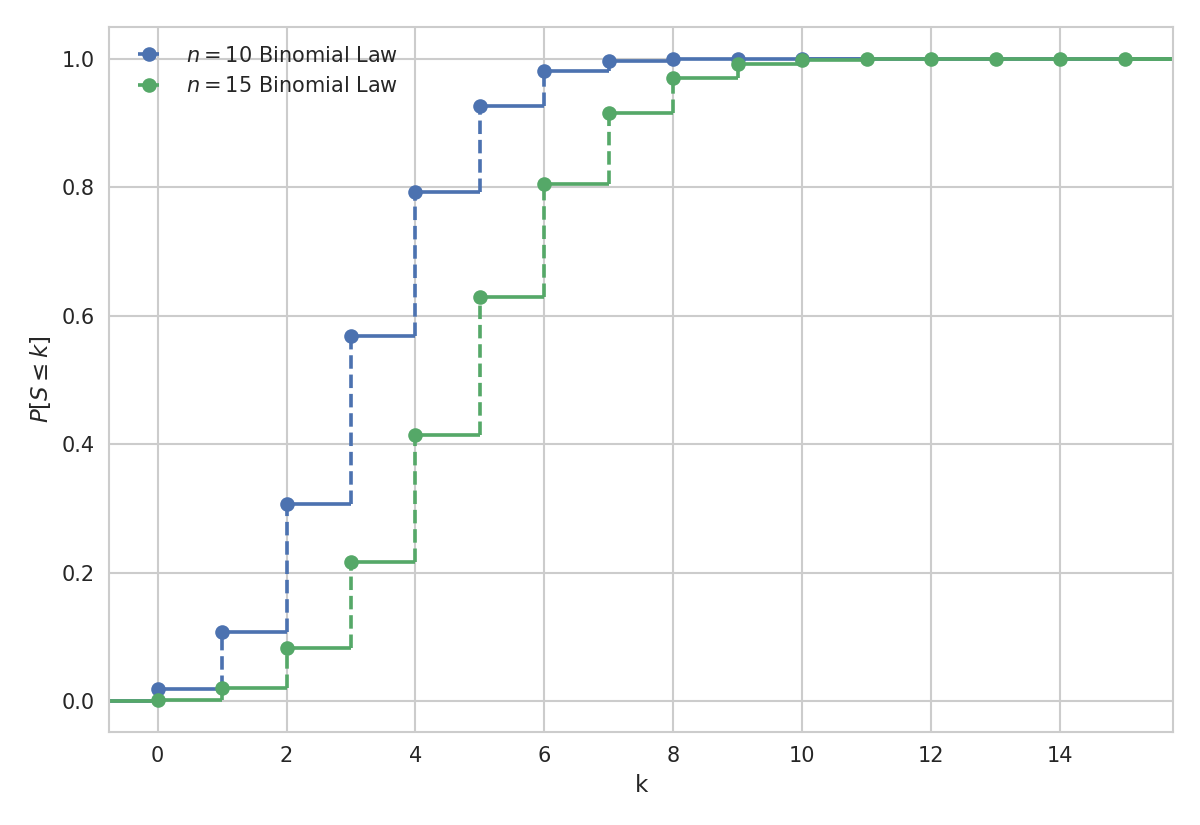
\includegraphics[scale=.5]{plot-discrete-binomapprox.png}


\subsubsection{$>50\%$ Fail}
A number under which more than fifty percent of players fail for 10 and 15 respectively are 3 and 5.

\subsubsection{$>90\%$ Succeed}
The minimum number of dots that will show for $>90\%$ of rolls. For 10 and 15 are 1 and 2.

\end{document}










